\documentclass[tikz, border=5pt]{standalone}

\begin{document}
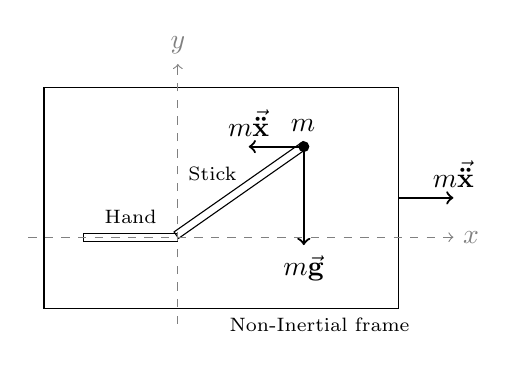
\begin{tikzpicture}

    %% FBD of the stick

    % Stick
    \begin{scope}[rotate=35]
        \draw (-1, -0.05) rectangle (1, 0.05);
        \node [above] at (1, 0.05) {\( m \)};
        \node [above] at (-0.3, 0.2) {\scriptsize Stick};
    \end{scope}

    % Gravitational force
    \draw[thick, ->] (0.8, 0.55) -- (0.8, -0.7) node[below] {\( m\vec{\mathbf{g}} \)};
    \fill (0.8, 0.55) circle (0.07);

    % Pseudo force
    \draw[thick, ->] (0.8, 0.55) -- (0.1, 0.55) node[above] {\( m\vec{\mathbf{\ddot x}} \)};

    % Hand
    \draw (-2, -0.55) rectangle (-0.8, -0.65);
    \node [above] at (-1.4, -0.55) {\scriptsize Hand};

    % Border frame
    \draw (-2.5, 1.3) rectangle (2, -1.5);

    % Inertial frame pseudo force
    \draw[thick, ->] (2, -0.1) -- (2.7, -0.1) node[above] {\( m\vec{\mathbf{\ddot x}} \)};
    \node [below] at (1, -1.5) {\scriptsize Non-Inertial frame};

    % Axes
    \draw[->, dashed, gray] (-0.8, -1.7) -- (-0.8, 1.6) node[above] {\( y \)};
    \draw[->, dashed, gray] (-2.7, -0.6) -- (2.7, -0.6) node[right] {\( x \)};

\end{tikzpicture}
\end{document}
